\section{Methods}
\label{sec:methods}

The analysis applies three complementary methods: unsupervised
regime discovery to test hypothesis H1, supervised walk-forward
forecasting with SHAP interpretability to test hypotheses H2, H3, and
H4, and a curated NLP corpus that overlays qualitative event context
on top of the quantitative model.

\begin{figure}[H]
\centering
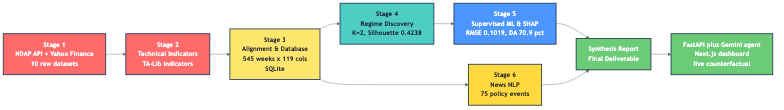
\includegraphics[width=\linewidth]{../diagram/pipeline_overview.png}
\caption{Project pipeline at a glance. Stages run sequentially in the
order shown; each stage is idempotent and reads only from the previous
stage's persisted output.}
\label{fig:pipeline-overview}
\end{figure}

\subsection{Unsupervised regime discovery}
\label{sec:methods-regimes}

\textbf{Implementation.} \texttt{scripts/stage4\_regime_discovery.py}.

The unsupervised stage takes the 86-column numeric feature matrix
(target and target lags excluded), applies \texttt{StandardScaler} for
zero mean and unit variance, then PCA. Fourteen principal components
retain 90.4\% of the total variance and are passed to a K-Means sweep
across $K = 2$ to $K = 7$. The chosen metric is the silhouette score,
which measures how tight each cluster is relative to its nearest
neighbour cluster.

\begin{table}[H]
\caption{K-Means silhouette sweep. K=2 is selected on both the
silhouette criterion and the macroeconomic interpretability criterion.}
\label{tab:silhouette-sweep}
\renewcommand{\arraystretch}{1.18}
\rowcolors{2}{SoftGray}{white}
\begin{tabular}{@{} l c l @{}}
\toprule
\rowcolor{Slate}\color{white}\textbf{K} &
\color{white}\textbf{Silhouette score} &
\color{white}\textbf{Notes} \\
\midrule
\textbf{2} & \textbf{0.4238} & \textbf{Optimal, aligns with COVID structural break} \\
3 & 0.4048 & Splits Regime 0 into COVID-peak and post-COVID, no clear policy boundary \\
4 & 0.3321 & Over-fragmentation \\
5 & 0.3351 & Over-fragmentation \\
6 & 0.3205 & Over-fragmentation \\
7 & 0.3022 & Over-fragmentation \\
\bottomrule
\end{tabular}
\end{table}

\begin{figure}[H]
\centering
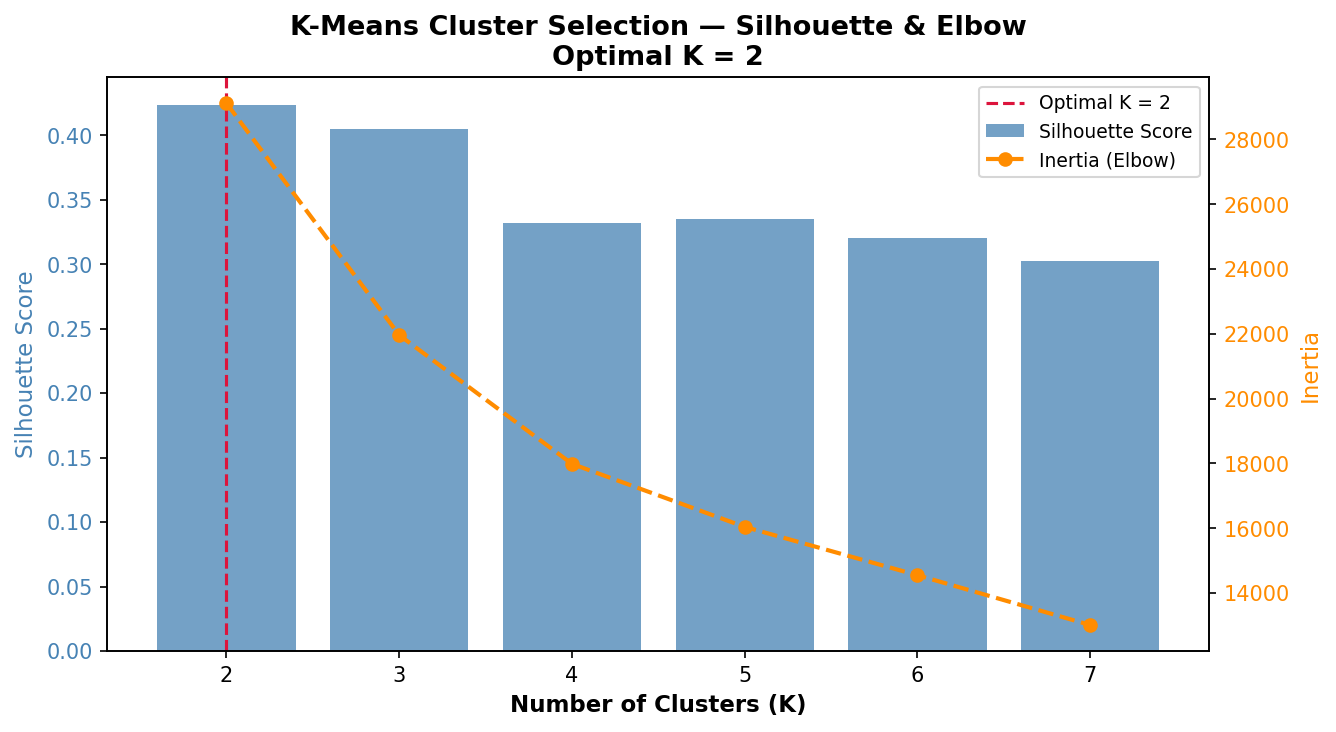
\includegraphics[width=0.78\linewidth]{../../visualizations/silhouette_scores.png}
\caption{Silhouette score across K. K=2 is optimal by a margin
over K=3 (0.0190), but K=2 cleanly aligns with the COVID structural
break while K=3's extra split does not align with any known policy
discontinuity.}
\label{fig:silhouette}
\end{figure}

\begin{figure}[H]
\centering
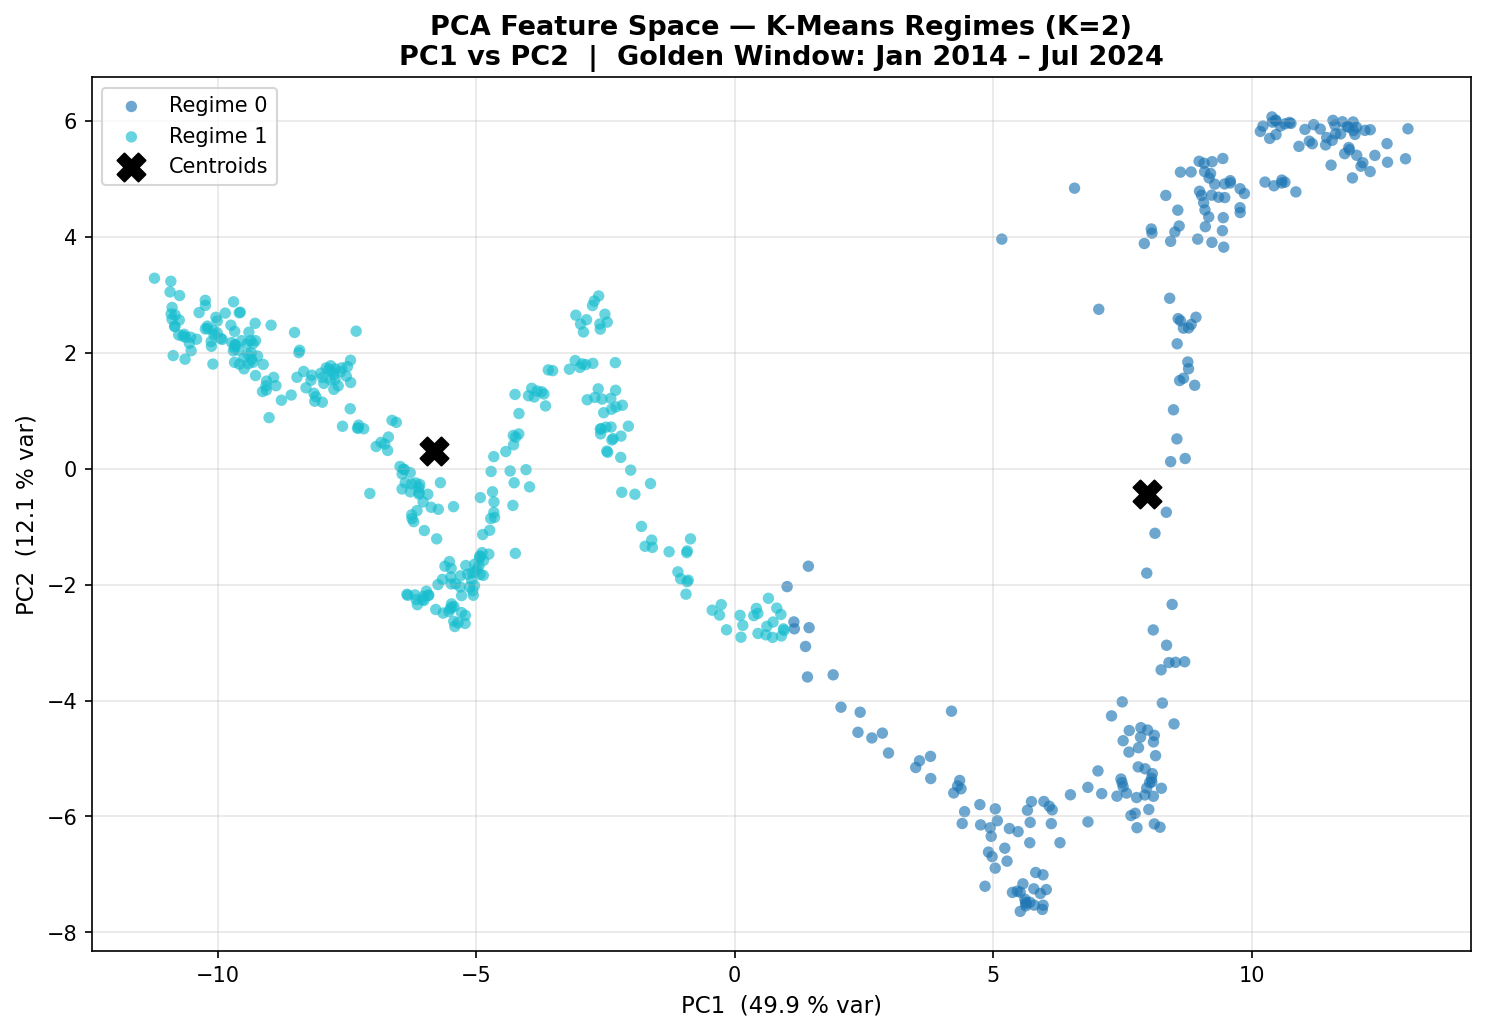
\includegraphics[width=0.92\linewidth]{../../visualizations/pca_regime_scatter.png}
\caption{Two-dimensional PCA projection of all 545 weeks, coloured by
the K=2 cluster assignment. The two clusters are visually
well-separated along PC1.}
\label{fig:pca-scatter}
\end{figure}

\begin{figure}[H]
\centering
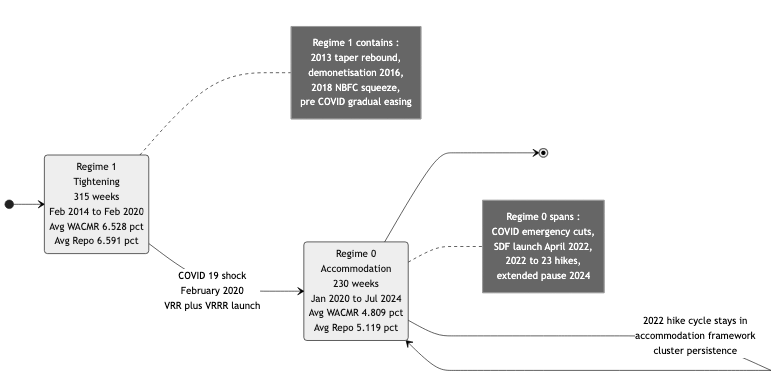
\includegraphics[width=\linewidth]{../diagram/regime_state_machine.png}
\caption{Discovered regimes as a state machine. The model identifies
two non-overlapping macroeconomic states with a single transition at
the COVID-19 shock in early 2020.}
\label{fig:regime-state-machine}
\end{figure}

\textbf{Discovered regimes.} The K=2 fit produces two clean clusters
that correspond to recognisable macroeconomic regimes:

\begin{itemize}
\item \textbf{Regime 1, Tightening:} 315 weeks from February 2014 to
  February 2020, with mean WACMR 6.528\%, mean Repo 6.591\%, and mean
  MSF 7.149\%. This regime contains the post-2013 taper-tantrum
  recovery, demonetisation in November 2016, and the gradual easing
  toward 5.15\% by late 2019.
\item \textbf{Regime 0, Accommodation:} 230 weeks from January 2020
  to July 2024, with mean WACMR 4.809\%, mean Repo 5.119\%, and mean
  MSF 5.369\%. This regime spans the COVID emergency rate cuts, the
  introduction of VRR and VRRR liquidity operations, the SDF launch
  in April 2022, and the subsequent 2022--2023 hiking cycle. The
  cluster correctly identifies that even post-COVID rate hikes still
  operate inside a structurally different liquidity-management
  framework than the pre-2020 normal.
\end{itemize}

\begin{figure}[H]
\centering
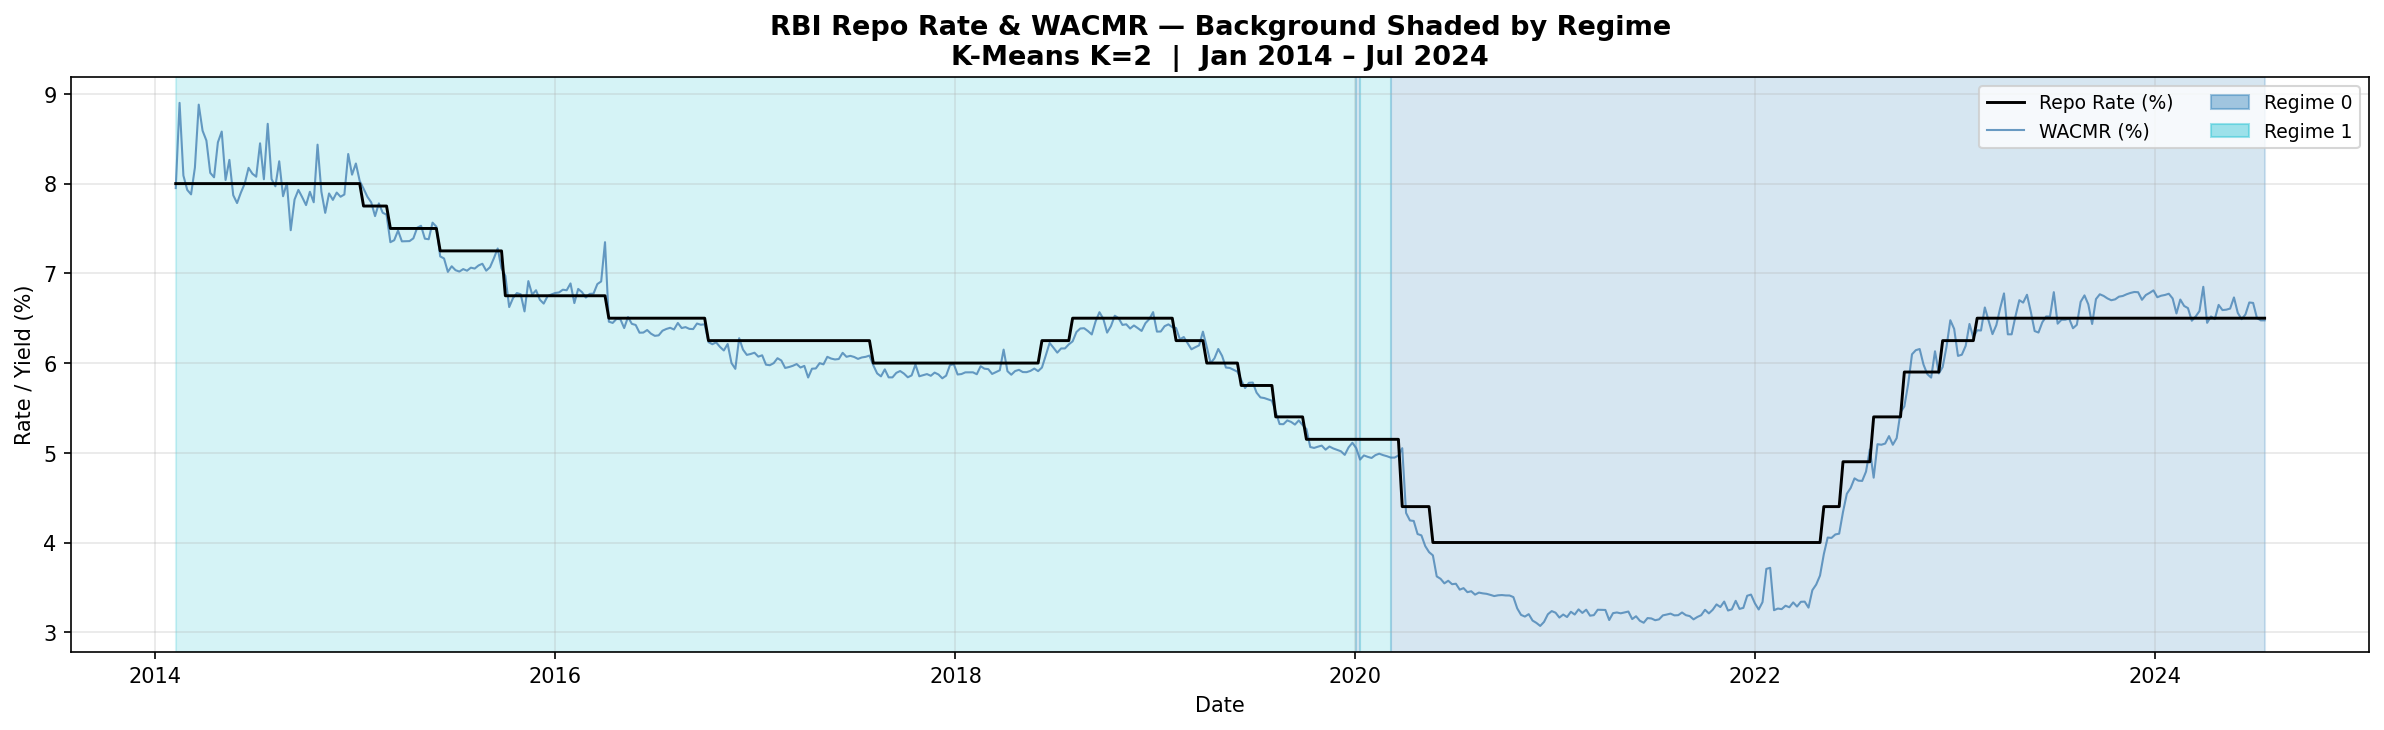
\includegraphics[width=\linewidth]{../../visualizations/regime_timeseries.png}
\caption{WACMR weekly time series with regime shading. The clean break
in early 2020 is visible as both a colour change and a shift in level.}
\label{fig:regime-timeseries}
\end{figure}

\begin{figure}[H]
\centering
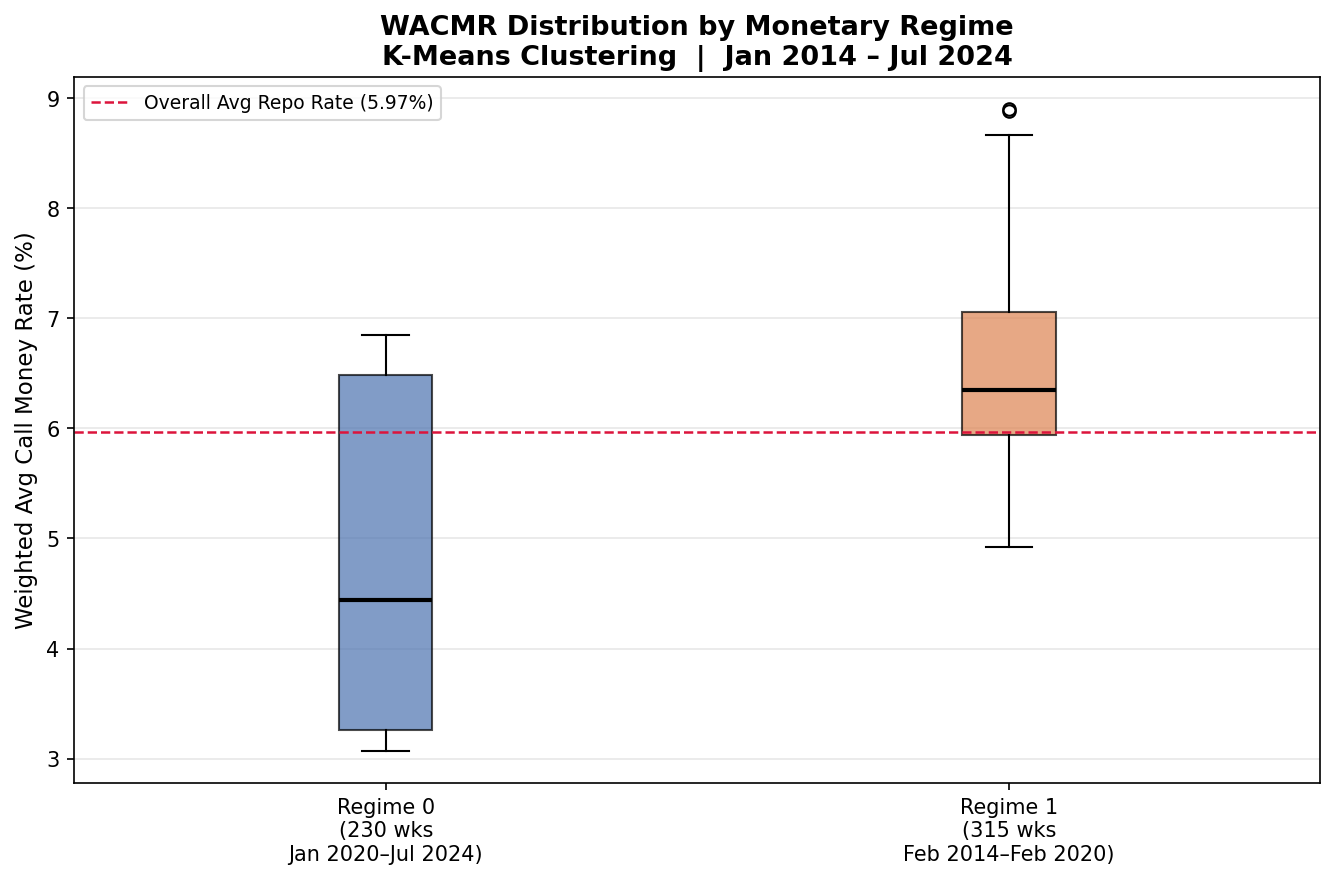
\includegraphics[width=0.78\linewidth]{../../visualizations/regime_wacmr_boxplot.png}
\caption{WACMR distribution by regime. The two distributions are
nearly disjoint, with only minor overlap in the 5.0--5.5\% band.}
\label{fig:regime-boxplot}
\end{figure}

\textbf{Interpretation.} Hypothesis H1 is supported. The data alone,
without any human labelling of dates, identifies two statistically
distinct regimes. The transition aligns precisely with the COVID-19
shock and the corresponding shift in RBI's liquidity-management
framework.

\subsection{Supervised forecasting}
\label{sec:methods-supervised}

\textbf{Implementation.} \texttt{scripts/stage5\_supervised\_ml.py}.

\subsubsection{Cross-validation protocol}

The supervised stage uses a strict walk-forward expanding-window
cross-validation, which is the appropriate choice for time-series
forecasting because it preserves temporal ordering and forbids
look-ahead. The training window starts at the first 156 weeks (three
years) and grows by one week per fold; in each fold the model is
trained on weeks 1 to $t$ and evaluated on week $t+1$. This procedure
yields 389 single-step out-of-sample predictions in total.

\begin{figure}[H]
\centering
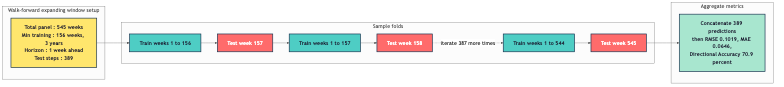
\includegraphics[width=\linewidth]{../diagram/walkforward_cv.png}
\caption{Walk-forward expanding-window cross-validation. Each fold
trains on all data up to week $t$ and is evaluated on week $t+1$.
389 folds in total.}
\label{fig:walkforward}
\end{figure}

\subsubsection{Model and hyperparameters}

The base estimator is \texttt{xgboost.XGBRegressor} (xgboost v2.1.4)
with a fixed set of hyperparameters chosen for low variance and
moderate regularisation. The choice was validated by a brief grid
search on the first 156 weeks, which is reported in the project
notebooks.

\begin{table}[H]
\caption{XGBoost hyperparameters used throughout the walk-forward
evaluation.}
\renewcommand{\arraystretch}{1.18}
\rowcolors{2}{SoftGray}{white}
\begin{tabularx}{0.8\linewidth}{@{} l Y l @{}}
\toprule
\rowcolor{Slate}\color{white}\textbf{Hyperparameter} &
\color{white}\textbf{Description} &
\color{white}\textbf{Value} \\
\midrule
\texttt{n\_estimators} & Number of boosted trees & 400 \\
\texttt{learning\_rate} & Shrinkage applied to each tree & 0.05 \\
\texttt{max\_depth} & Maximum tree depth & 4 \\
\texttt{subsample} & Row subsampling per tree & 0.8 \\
\texttt{colsample\_bytree} & Column subsampling per tree & 0.8 \\
\texttt{reg\_alpha} & L1 regularisation strength & 0.1 \\
\texttt{reg\_lambda} & L2 regularisation strength & 1.0 \\
\bottomrule
\end{tabularx}
\end{table}

\subsubsection{Two model variants}

Two variants are evaluated under the identical walk-forward protocol.
The baseline uses 117 features (the corridor rates, the balance-sheet
items, the debt-market and CPI columns, the OHLCV plus indicator
columns from Stage 1b, and three engineered spreads, plus three
autoregressive lags of the target). The regime-aware variant adds
five further columns: two one-hot regime indicators and two
PCA-space distances to the K-Means centroids, for a total of 122
features.

\begin{table}[H]
\caption{Out-of-sample performance over 389 walk-forward test weeks.
Baseline wins on RMSE; both variants tie on MAE and directional
accuracy. Hypothesis H2 is rejected.}
\label{tab:perf}
\renewcommand{\arraystretch}{1.2}
\rowcolors{2}{SoftGray}{white}
\begin{tabularx}{\linewidth}{@{} Y c c c @{}}
\toprule
\rowcolor{Slate}\color{white}\textbf{Metric} &
\color{white}\textbf{Baseline (89 features)} &
\color{white}\textbf{Regime-aware (94 features)} &
\color{white}\textbf{Change} \\
\midrule
RMSE & \textbf{0.1019} & 0.1044 & $+2.5\%$ \\
MAE & 0.0646 & 0.0646 & $0.0\%$ \\
Directional accuracy & 70.9\% & 70.9\% & $+0.0$pp \\
\bottomrule
\end{tabularx}
\end{table}

\begin{figure}[H]
\centering
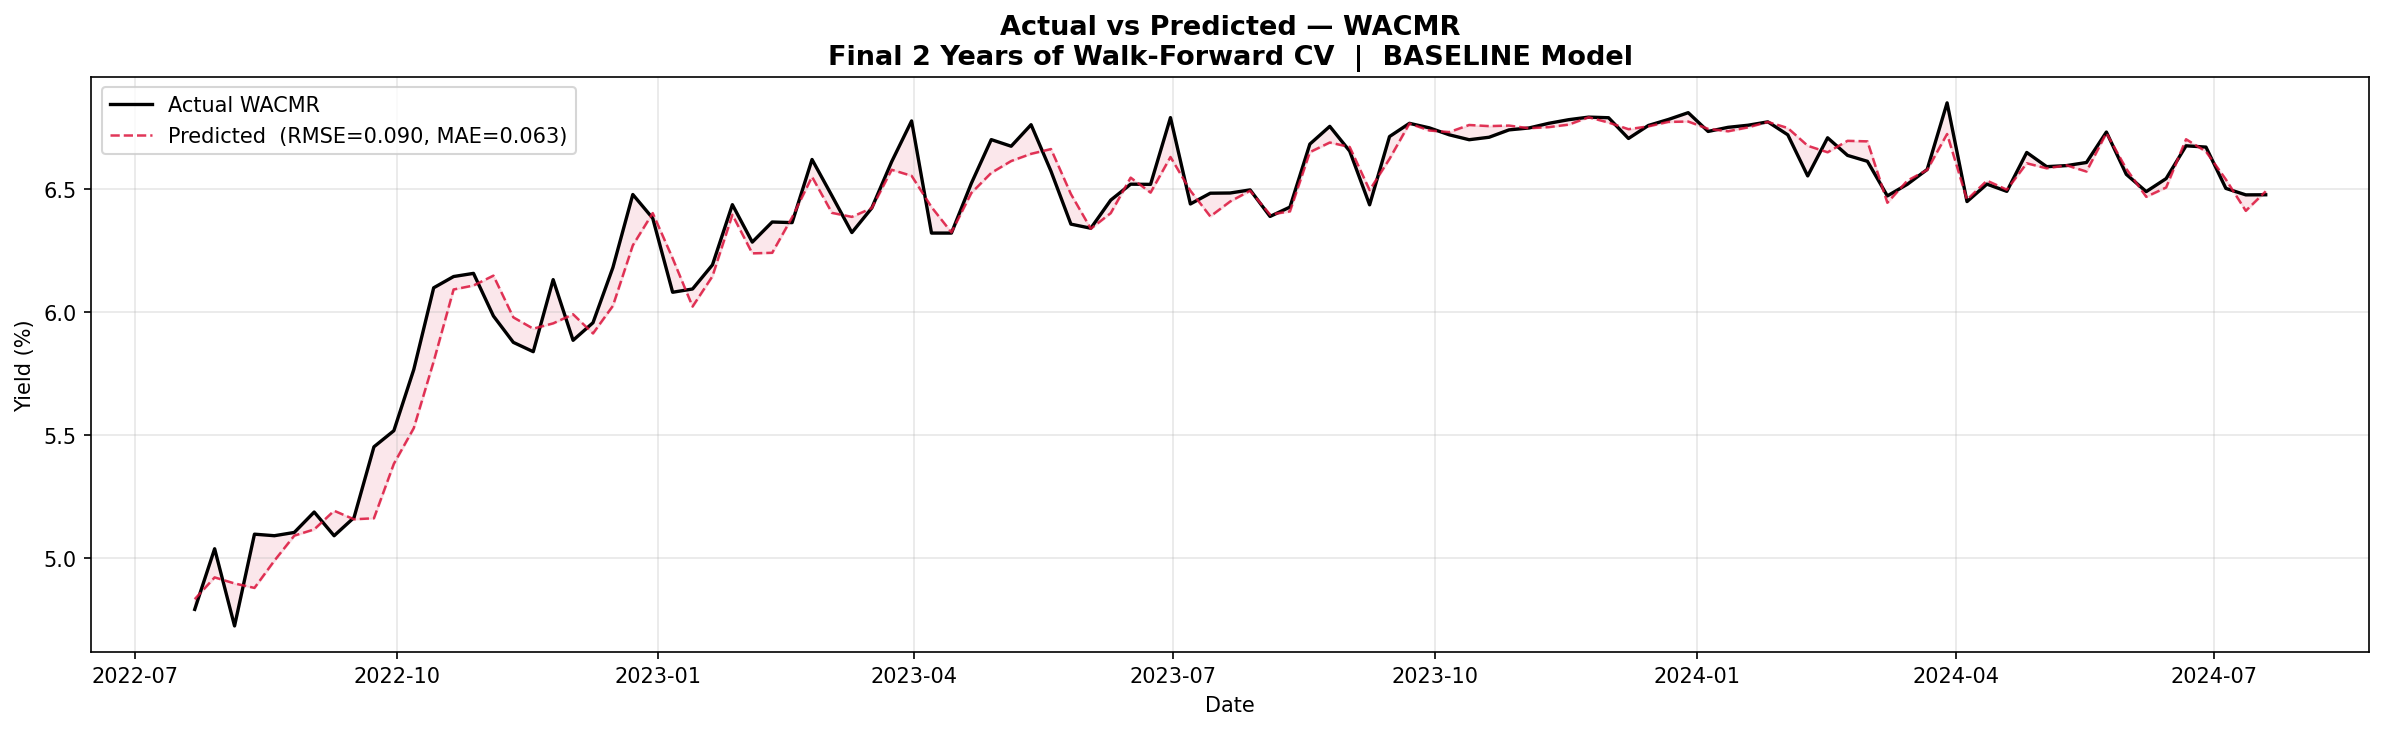
\includegraphics[width=\linewidth]{../../visualizations/actual_vs_predicted.png}
\caption{Actual versus predicted WACMR over the 389 walk-forward test
weeks. The model tracks the level closely outside of three large
unpredictable policy actions in 2020 and 2022.}
\label{fig:actual-vs-predicted}
\end{figure}

\textbf{Interpretation.} Hypothesis H2 is rejected. The baseline
model already learns the regime structure implicitly through the
lagged Repo Rate and the autoregressive lags of WACMR; adding
explicit regime labels provides redundant signal that mildly worsens
RMSE without any gain on MAE or directional accuracy. This is
genuinely informative rather than disappointing: it tells us that an
XGBoost regressor with the right features needs no help recovering
the regime structure of Indian monetary policy from the data alone.

\subsubsection{SHAP interpretability}

SHAP values are computed for every test prediction with
\texttt{shap.TreeExplainer}, which exploits the tree structure of the
fitted XGBoost model to attribute the difference between each
prediction and the model's baseline expectation to individual
features. Mean absolute SHAP values across the 545 weeks give a
global feature-importance ranking.

\begin{figure}[H]
\centering
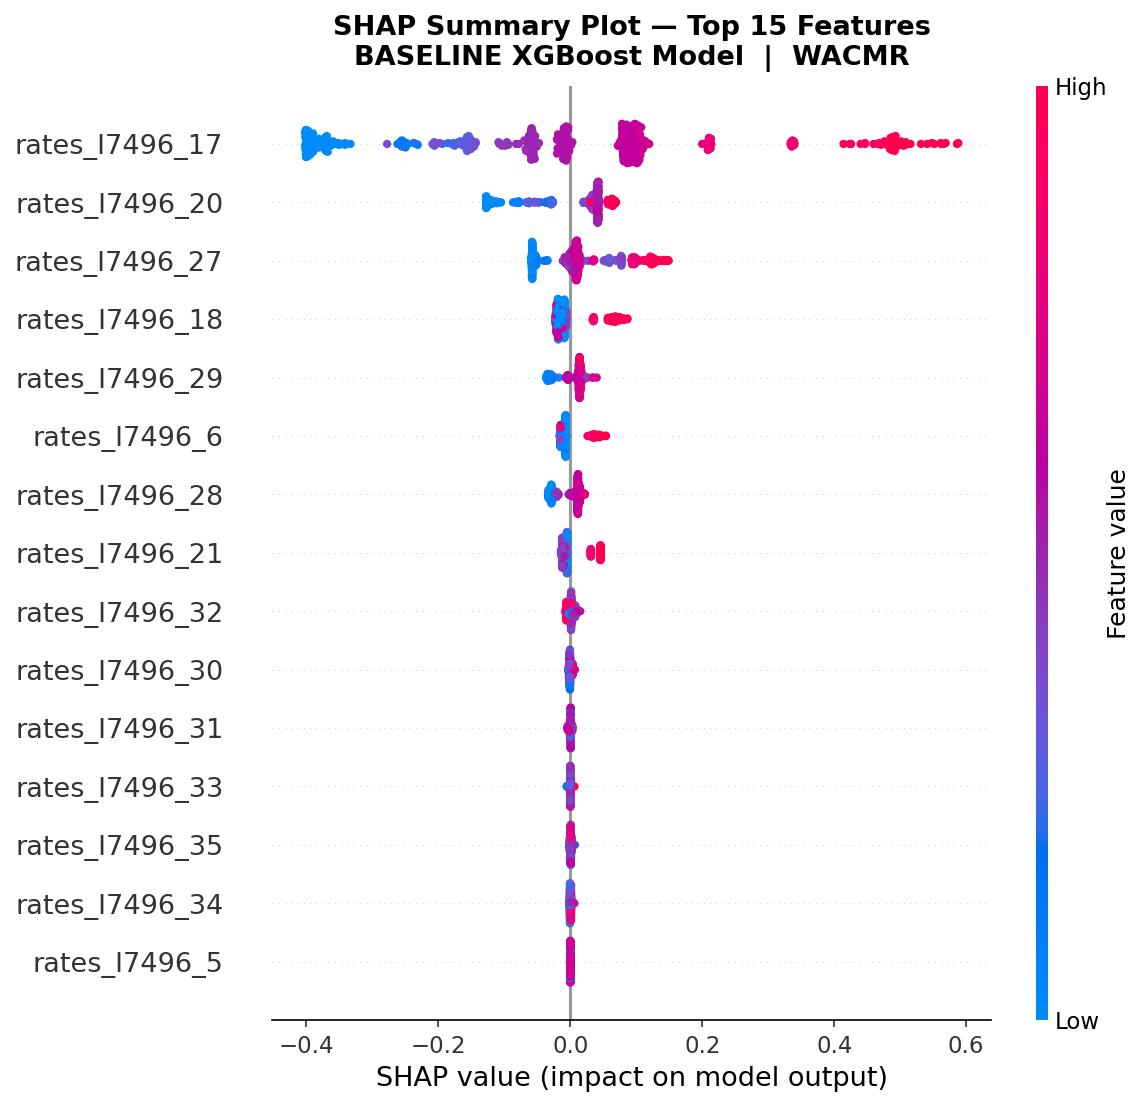
\includegraphics[width=\linewidth]{../../visualizations/shap_summary.png}
\caption{SHAP feature-importance summary, top 15 features by mean
absolute SHAP value. The five highest features are all rate-corridor
or autoregressive variables.}
\label{fig:shap-summary}
\end{figure}

\begin{table}[H]
\caption{SHAP top 15 features. The corridor rates and the
autoregressive lags of WACMR fill the entire top-15 list. None of the
twenty-eight equity or forex features cracks the threshold.}
\label{tab:shap-top15}
\renewcommand{\arraystretch}{1.16}
\rowcolors{2}{SoftGray}{white}
\begin{tabularx}{\linewidth}{@{} c l l c Y @{}}
\toprule
\rowcolor{Slate}\color{white}\textbf{Rank} &
\color{white}\textbf{Feature} &
\color{white}\textbf{Group} &
\color{white}\textbf{Mean $|$SHAP$|$} &
\color{white}\textbf{Plain reading} \\
\midrule
1  & \texttt{target\_lag1}            & autoregressive    & 0.48959 & WACMR last week \\
2  & \texttt{repo\_lag1}              & autoregressive    & 0.21053 & Repo Rate last week \\
3  & \texttt{rates\_I7496\_17}        & policy corridor   & 0.19459 & Current Repo Rate \\
4  & \texttt{spread\_wacmr\_minus\_repo} & engineered     & 0.07247 & Liquidity stress proxy \\
5  & \texttt{rates\_I7496\_20}        & policy corridor   & 0.05847 & MSF Rate, upper bound \\
6  & \texttt{target\_lag2}            & autoregressive    & 0.05047 & WACMR two weeks ago \\
7  & \texttt{repo\_lag4}              & autoregressive    & 0.04951 & Repo Rate four weeks ago \\
8  & \texttt{rates\_I7496\_27}        & overnight rates   & 0.04074 & CBLO/Tri-party Repo \\
9  & \texttt{target\_lag4}            & autoregressive    & 0.02238 & WACMR four weeks ago \\
10 & \texttt{rates\_I7496\_18}        & policy corridor   & 0.02068 & Reverse Repo, lower bound \\
11 & \texttt{rates\_I7496\_29}        & money market      & 0.01734 & CD Rate \\
12 & \texttt{rates\_I7496\_6}         & structural        & 0.01694 & SLR \\
13 & \texttt{rates\_I7496\_28}        & money market      & 0.01619 & Market Repo Rate \\
14 & \texttt{rates\_I7496\_21}        & policy corridor   & 0.01362 & Bank Rate \\
15 & \texttt{la\_I7492\_15}           & balance sheet     & 0.01124 & RBI balance-sheet item \\
\bottomrule
\end{tabularx}
\end{table}

\begin{finding}
The first three SHAP features alone (\texttt{target\_lag1},
\texttt{repo\_lag1}, current Repo Rate) account for the majority of
the model's predictive power, with combined mean absolute SHAP value
of 0.89471 against a total over the top 15 of approximately 1.285. The
twenty-eight Nifty 50 and USD/INR features collectively contribute
less than the single SHAP value of \texttt{rates\_I7496\_15}.
Hypothesis H4 is rejected: equity and forex sentiment do not
materially improve WACMR forecasting at the weekly horizon.
Hypothesis H3 is supported: the policy corridor (Repo, Reverse Repo,
MSF) dominates the feature importance ranking.
\end{finding}

\subsubsection{Regime-conditional SHAP}

Splitting the 545 SHAP rows by regime label exposes a mechanical
difference in how the model operates inside each macroeconomic
environment.

\begin{figure}[H]
\centering
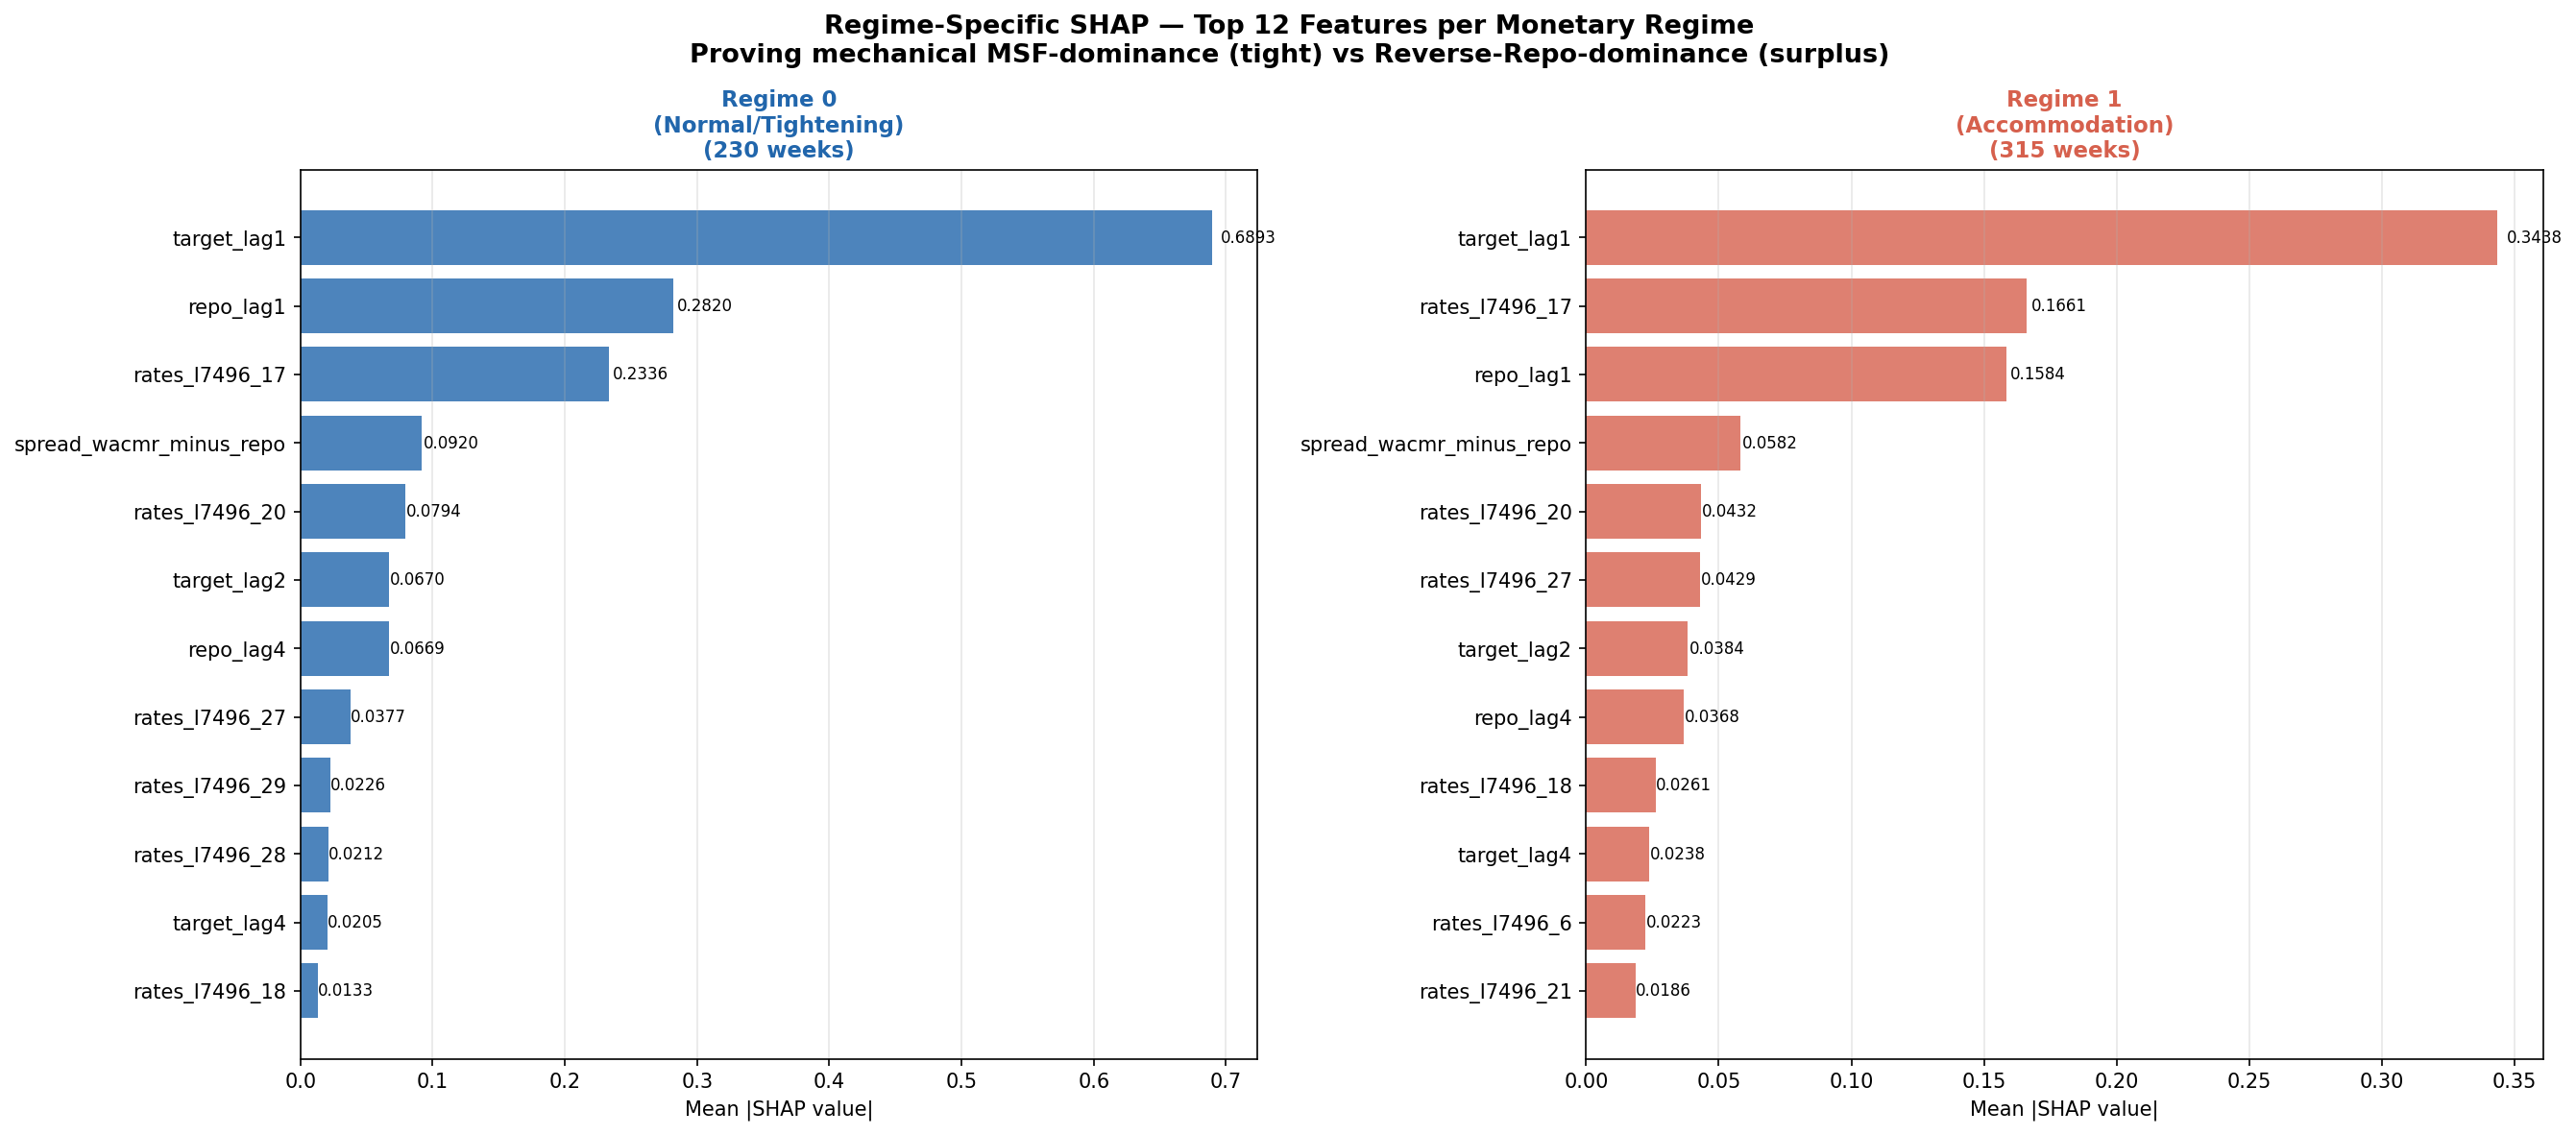
\includegraphics[width=\linewidth]{../../visualizations/shap_by_regime.png}
\caption{Top-12 SHAP feature importance, stratified by regime. Two
substantive shifts are visible: the Reverse Repo Rate rises from
rank 12 to rank 9 in the accommodation regime, and the absolute SHAP
magnitude of the autoregressive lag halves from Tightening to
Accommodation.}
\label{fig:shap-by-regime}
\end{figure}

Two substantive findings drop out of this comparison. First, the
Reverse Repo (and post-2022 the SDF) Rate rises sharply in importance
in the accommodation regime, which is exactly what monetary theory
predicts: in surplus liquidity conditions the binding constraint on
WACMR is the lower corridor floor rather than the upper ceiling.
Second, the absolute SHAP magnitude of every feature is roughly twice
as large in the tightening regime than in the accommodation regime
(\texttt{target\_lag1}'s SHAP value is 0.689 versus 0.344). This
quantifies the qualitative observation made in Section~\ref{sec:eda}:
WACMR is markedly more predictable from its own recent history during
tightening periods than during accommodation, when discretionary RBI
operations introduce more week-to-week noise.

\subsubsection{Residual analysis and calendar effects}

\begin{figure}[H]
\centering
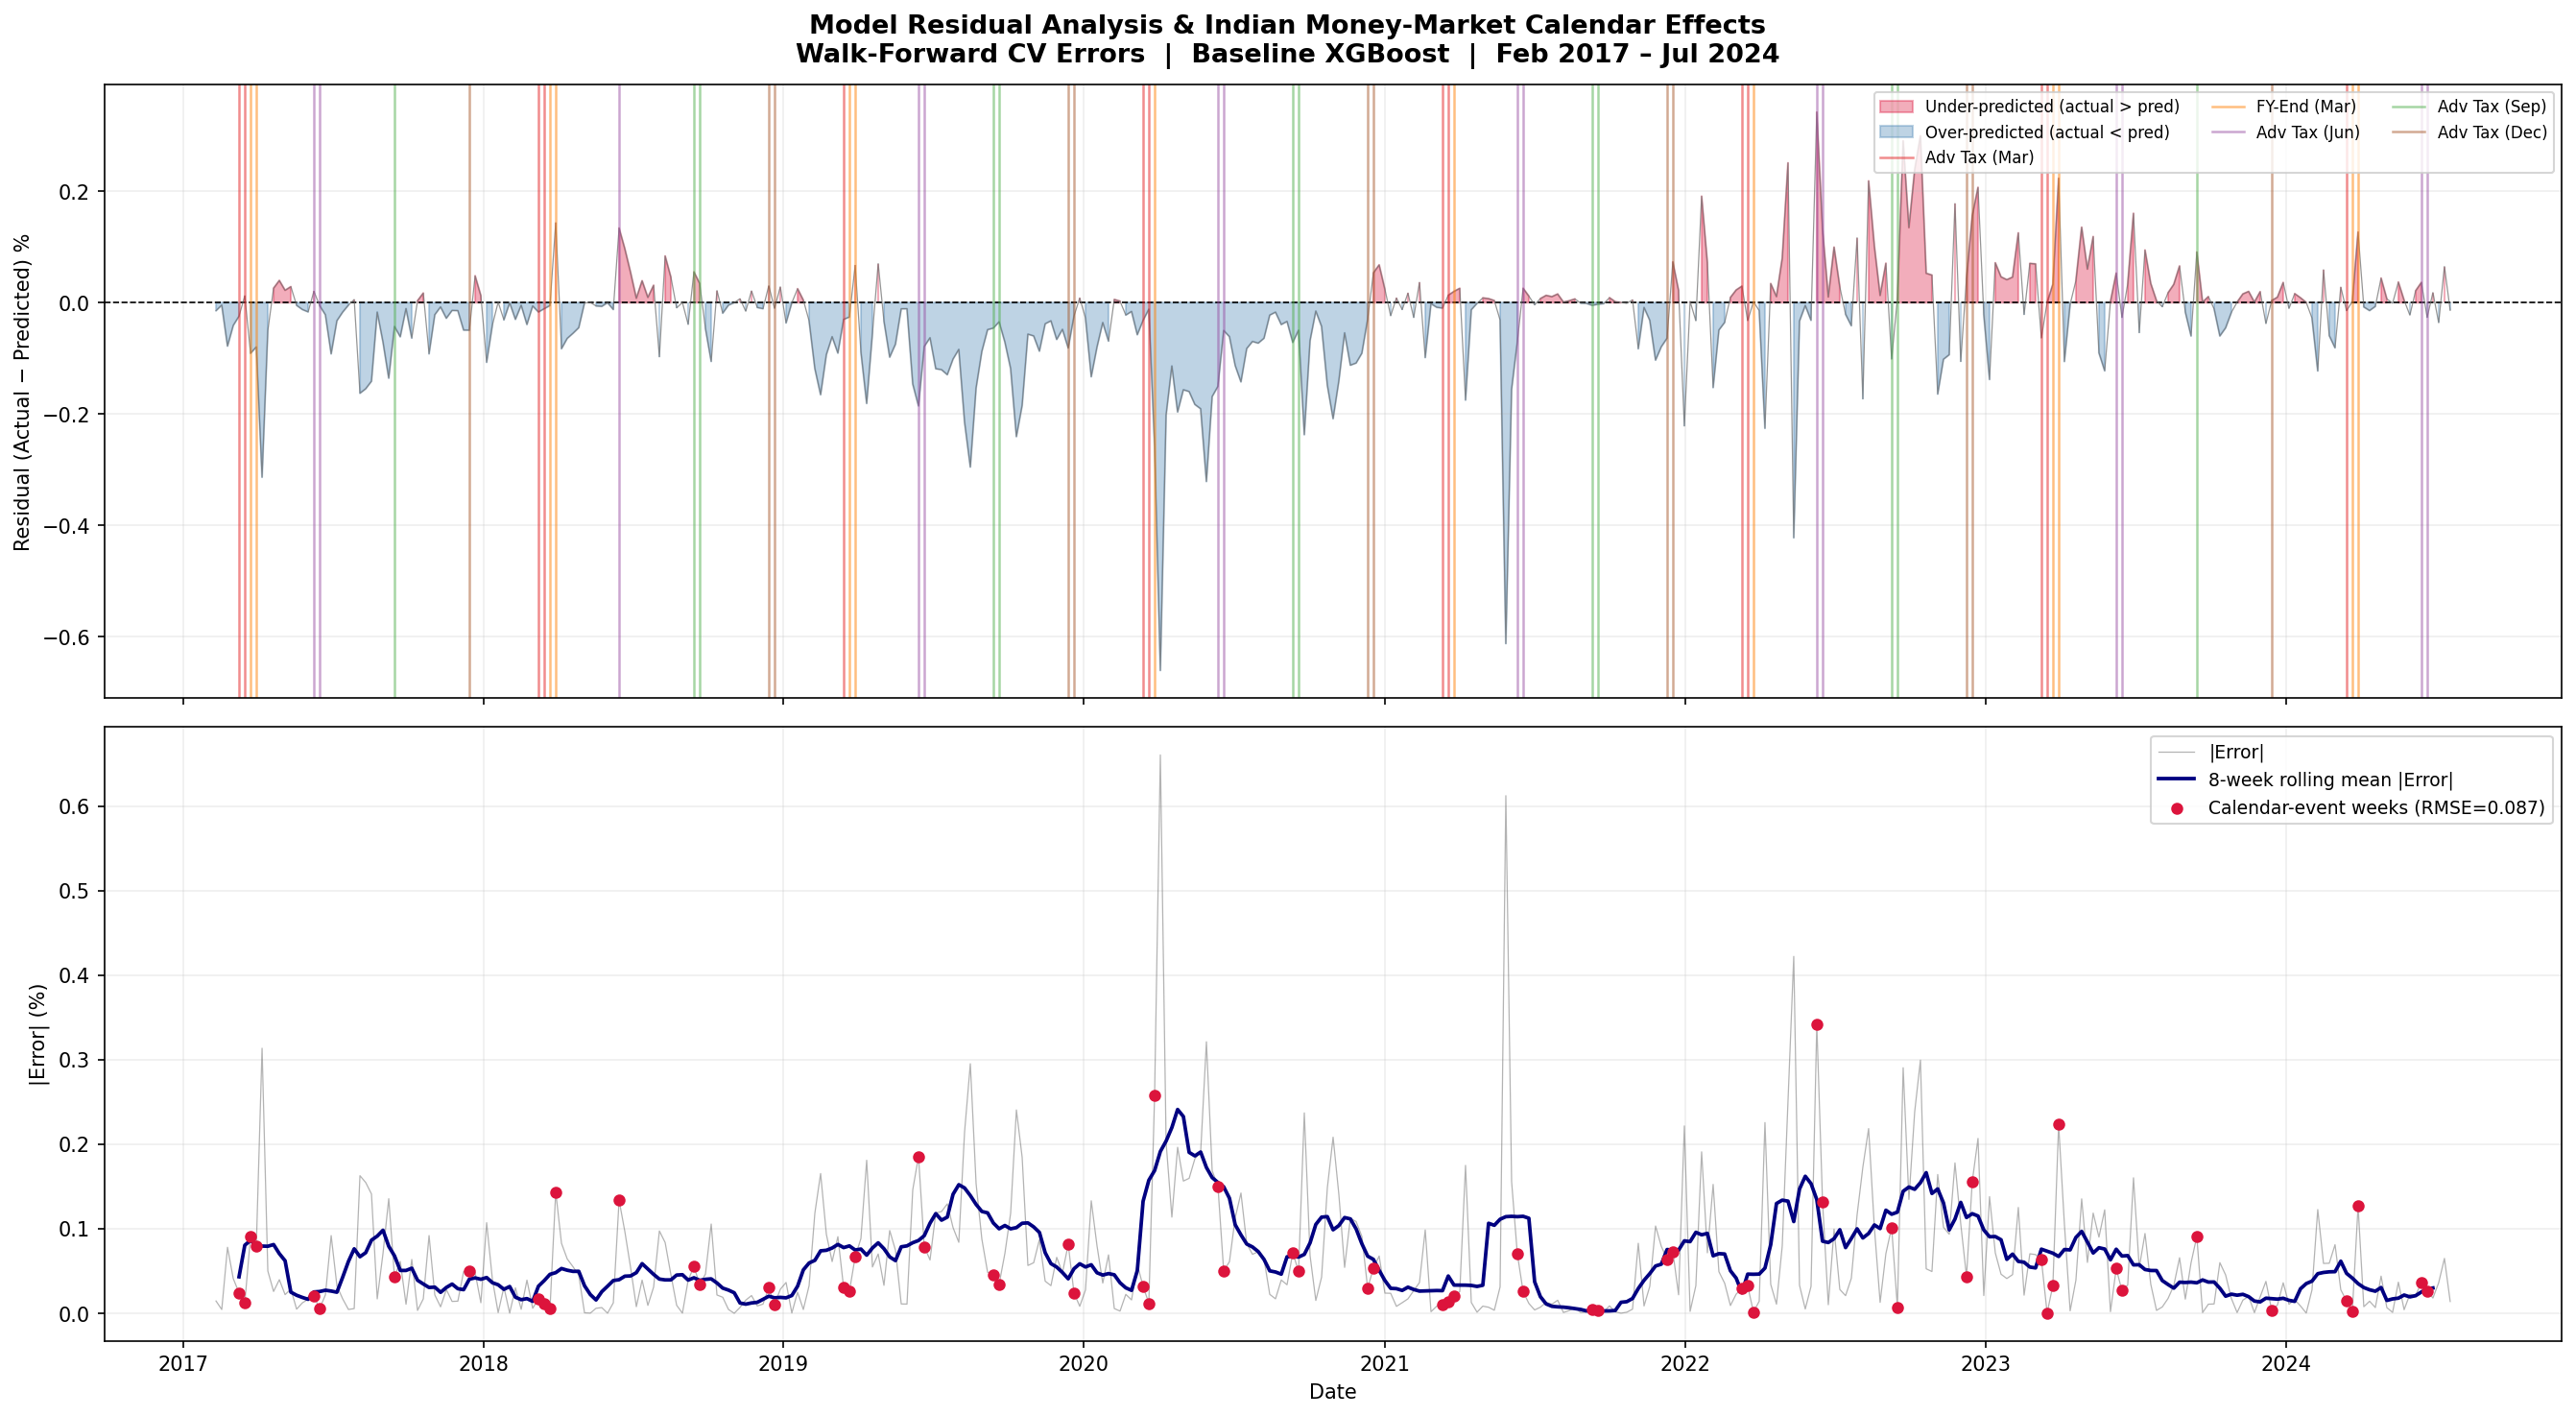
\includegraphics[width=\linewidth]{../../visualizations/residual_calendar.png}
\caption{Walk-forward residuals over time, with calendar-event weeks
(quarter-end, advance-tax dates, GST settlement) annotated. The
largest residuals are clustered around macro shocks, not around
calendar pressure.}
\label{fig:residual-calendar}
\end{figure}

A widely cited rule-of-thumb in Indian money-market research is that
the model's worst weeks should be financial-year end (March),
advance-tax outflow weeks (15 March, 15 June, 15 September, and
15 December), and GST settlement weeks. The residual analysis tests
this directly. Out of the 389 test weeks, 66 fall on calendar-event
dates. The model's RMSE on those weeks is 0.0870, which is
\textit{lower} than the 0.1046 RMSE on non-event weeks. The
calendar-effect hypothesis is rejected: ten years of training data is
sufficient for the model to learn the predictable seasonal patterns,
and the residual mass concentrates instead on a small number of
genuinely unpredictable macro shocks (the COVID emergency rate cut
on 3 April 2020, the surprise inter-meeting hike on 13 May 2022, and
the COVID second-wave peak in May--June 2021).

\subsection{NLP corpus and event analysis}
\label{sec:methods-nlp}

\textbf{Implementation.} \texttt{scripts/stage6\_news\_nlp.py}.

The NLP component takes a different shape from the supervised stage.
Rather than scraping a large body of text, the project curates a
focused corpus of seventy-five high-impact monetary-policy events
from February 2014 to August 2024. Each event has a date, a title, a
description, a category, an impact level, and a sentiment score in
$[-1, +1]$. Sentiment is positive for accommodative and dovish
actions (rate cuts, liquidity injections, reserve requirement cuts)
and negative for hawkish actions (rate hikes, liquidity absorption).

\begin{methodbox}
The choice to curate rather than scrape is deliberate. Off-the-shelf
sentiment models (VADER, FinBERT) trained on general financial
English routinely mis-classify Indian monetary-policy language; for
example, ``open market operation'' carries no sign in finance generally
but is a clear liquidity injection in the Indian context. With only
seventy-five events to annotate, expert curation produces cleaner
labels than any pre-trained model would, at acceptable cost. An
automated FinBERT pipeline over five years of RBI press releases is
identified as the natural future extension in
Section~\ref{sec:limitations}.
\end{methodbox}

\begin{figure}[H]
\centering
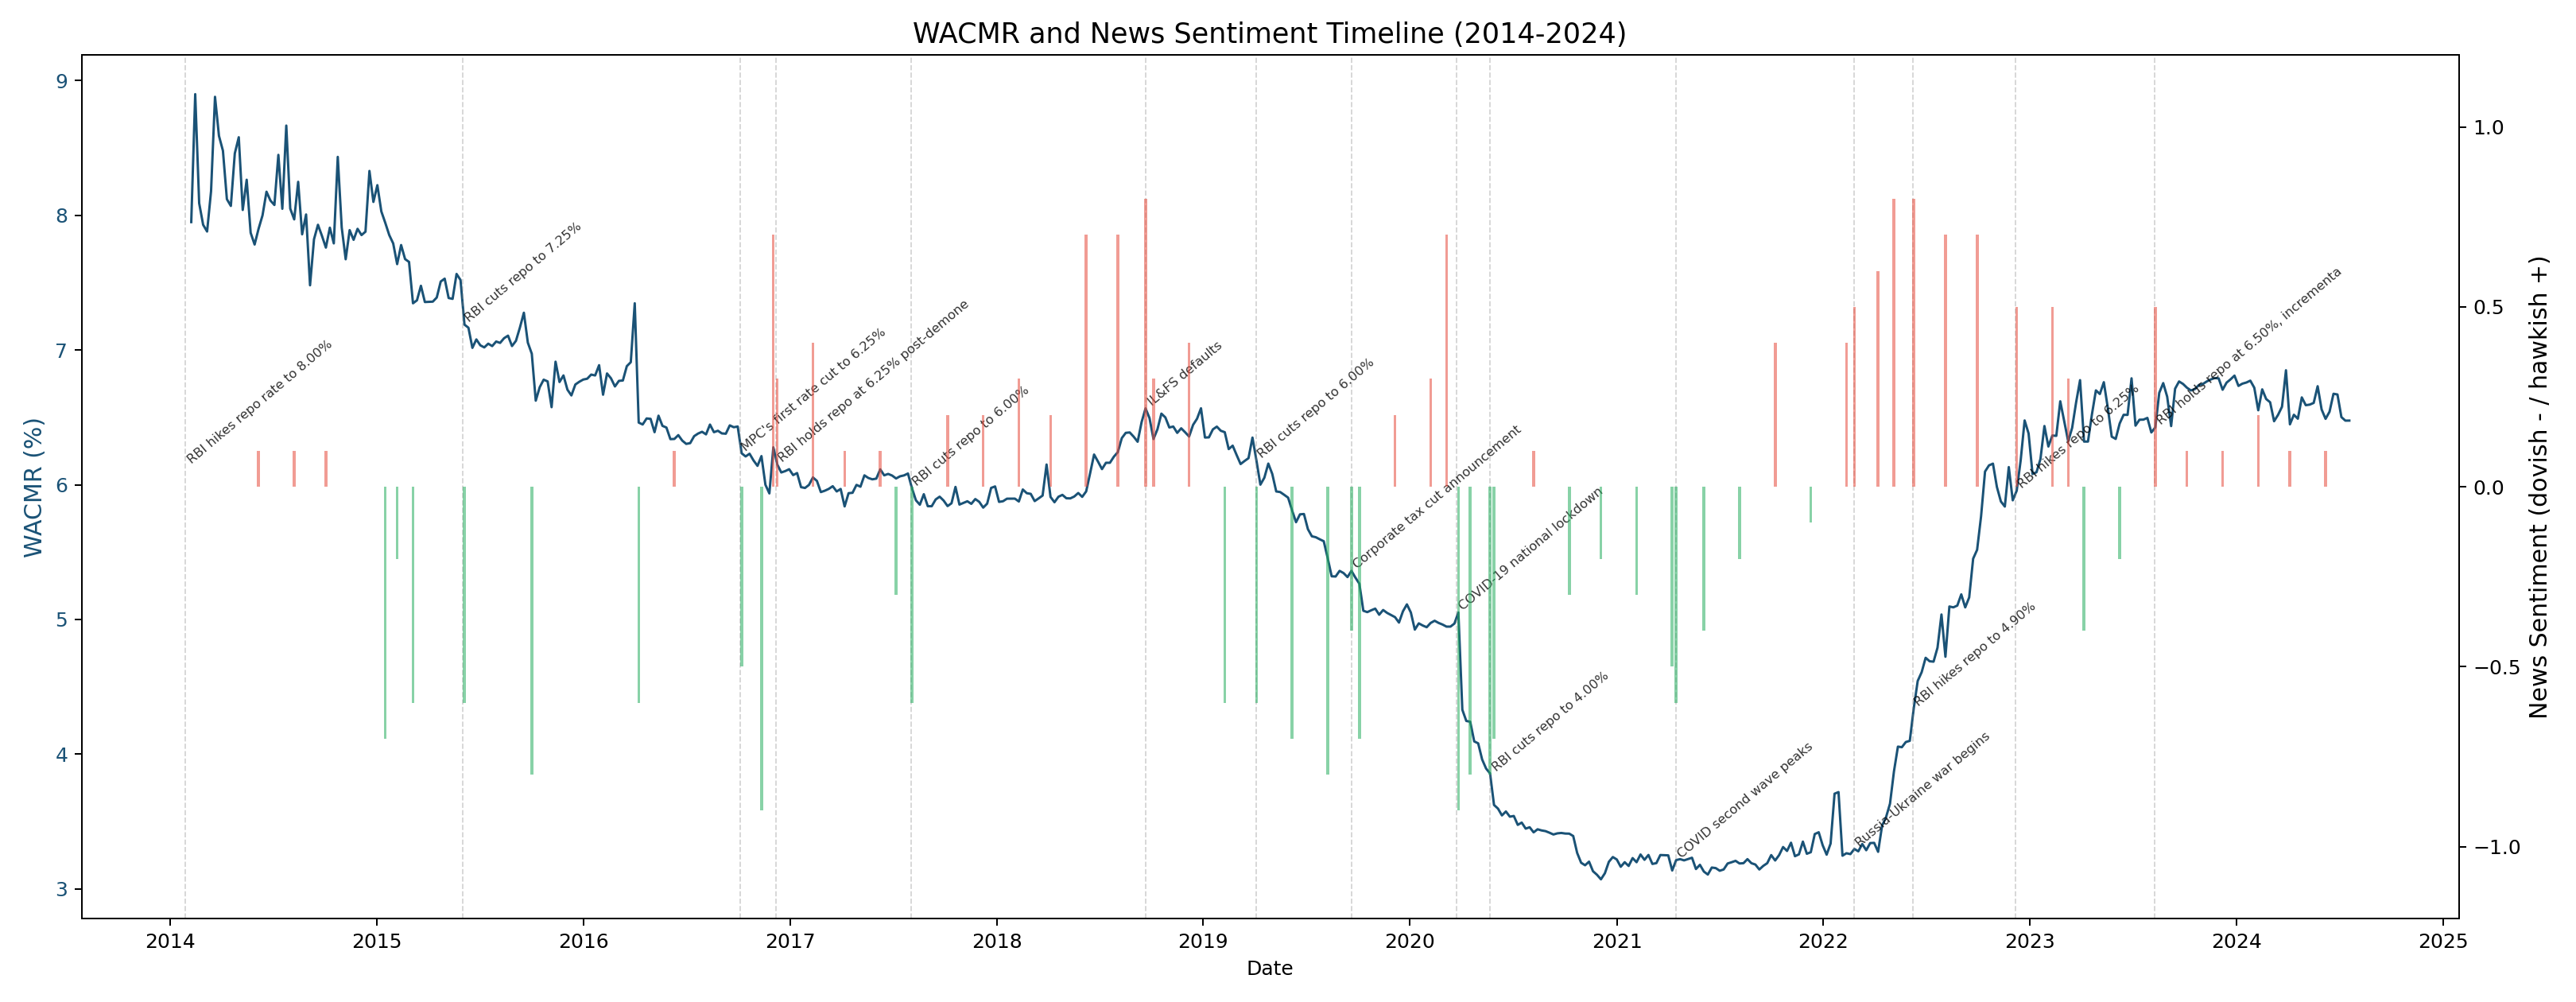
\includegraphics[width=\linewidth]{../../visualizations/news_sentiment_timeline.png}
\caption{Curated event sentiment over the analysis window. Positive
spikes cluster in 2020 around COVID accommodation; negative spikes
cluster in 2022--23 during the rate-hike cycle.}
\label{fig:news-sentiment}
\end{figure}

\begin{figure}[H]
\centering
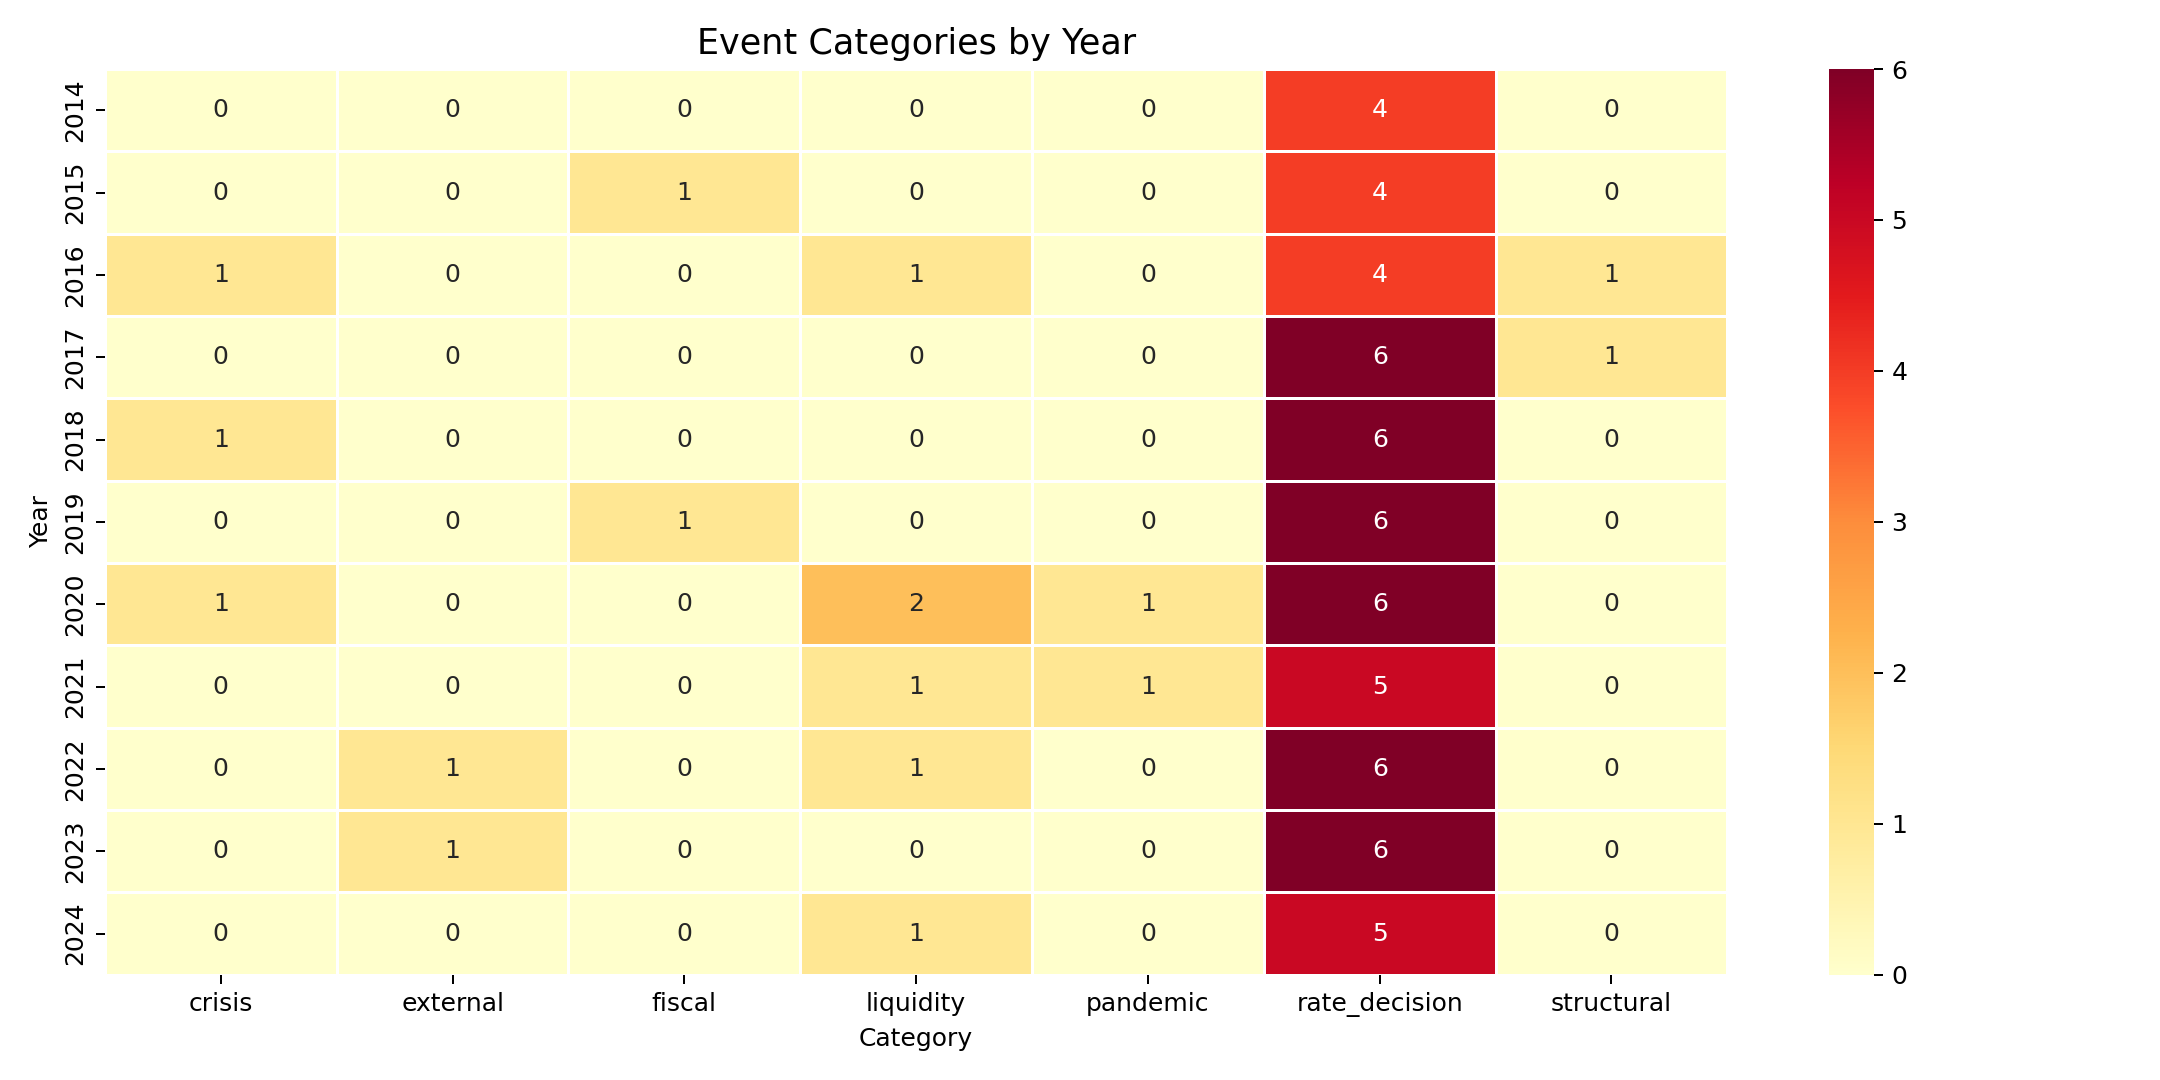
\includegraphics[width=\linewidth]{../../visualizations/event_density_heatmap.png}
\caption{Event density heatmap by category and time period. Crisis and
liquidity events concentrate around 2020; rate-decision events are
distributed throughout the window.}
\label{fig:event-density}
\end{figure}

The corpus is aggregated to weekly counts and mean sentiment, then
joined to the master panel. A downstream Pearson correlation between
weekly aggregate sentiment and the contemporaneous WACMR change
yields a small but interpretable $r = -0.21$: weeks with more
positive (dovish) policy actions are associated with downward WACMR
movements. The signal is too weak to use as a primary feature, but
the qualitative annotation it provides is useful for explaining
forecast errors, as shown by the alignment between the largest
residuals and the most negative-sentiment events in 2020 and 2022.
